\epigraph{ 
    This remark is based on a ``theorem'', which as far as I know has never been proven, but which I cannot imagine could be wrong.
}
{
    Steven Weinberg, 1979~\autocite{weinbergPhenomenologicalLagrangians1979a}
}


\section{Pion stars}

Stars and planets have long been one of the main driving engines behind the developments of physics.
A lot of early mathematics was developed to predict the seasons, the phases of the moon and to navigate using the stars.
One of the most important confirmation of Newton's laws of motion and gravity was their prediction of Kepler's laws, the empirical observations of the orbits of planets around the Sun.
Likewise, the successor to Newton's law of gravitation, Einstein's general relativity, was first shown to be more accurate than its predecessor by predicting the drift of the perihelion of the orbit of Mercury~\autocite{carrollSpacetimeGeometryIntroduction2019}.
The radiation of the Sun has been part of the development of the theory of light and thermal radiation~\autocite{hemmerTermiskFysikk2002}.
To understand the process that fuels the Sun, we had to develop special relativity, in which mass is described as just another form of energy, as well as quantum mechanics and the theory of nuclear fusion.
Observations of the neutrinos which result from these processes were used to show the process of neutrino oscillations~\autocite{prialnikIntroductionTheoryStellar2000}.
Today, these are some of the only empirical data in physics that conflict with the standard model of particle physics.
The Sun might therefore still be part of the development of new fundamental physics.

Even after a star has depleted its fusion fuel it can remain an object of great interest.
Stars with less mass than around $10$ times that of the earth, $M_\odot$, will towards the end of their active life shed most of their outer layers, leaving behind an inert white-hot mass only supported by the degeneracy pressure of electrons.
These are called \emph{white dwarves}.
One cubic centimeter of the material that makes up white dwarves weighs more than a ton.
Sirius B, the fainter companion to Sirius is a white dwarf.
Type Ia supernovae happen as white dwarves reach their upper mass limit, the Chandrasekhar limit, and are invaluable in mapping the distance of our universe~\autocite{carrollSpacetimeGeometryIntroduction2019}.
White dwarves, together with the even more dense \emph{neutron stars} collectively known as \emph{compact stars}.
Neutron stars are left after the supernova explosions of massive stars~\autocite{prialnikIntroductionTheoryStellar2000}.
They were first predicted solely on theoretical backgrounds, and later discovered in the form of pulsars, rotating neutron stars with frequencies below a tenth of a second which strong magnetic fields acting as particle accelerators~\autocite{prialnikIntroductionTheoryStellar2000},
Compact stars are some of the most environments in our universe, and as such, they are excellent places for exotic physics to happen.

Recently, a new form of compact stars has been proposed, called pion stars~\autocite{andersenBoseEinsteinCondensationPion2018,brandtNewClassCompact2018,carignanoScrutinizingPionCondensed2017}.
These stars are composed of a pion condensate.
The pion particles are bosons, in contrast to electrons and neutrons, which are fermions.
The pressure in pion stars must therefore be maintained by repulsive interactions, unlike in neutron stars and white dwarves, where it is due to the Pauli exclusion principle.
In this thesis, we will develop chiral perturbation theory (\chpt), a model for the dynamics of pions and the other pseudoscalar mesons, in order to investigate the properties of pion stars.
This involves a survey of the theoretical foundations and thermodynamic calculations.
Pion stars are, as yet, only a theoretical proposal.
However, if history is to be of any guidance, that does not mean there aren't valuable insights to be gained from researching them.
To that end, we need a theory of the matter that makes up such a star.




\section{The standard model, QCD, and effective theories}


The Standard Model of particle physics is the totality of what particle physicists are confident they understand concerning the fundamental building blocks of our universe.
It is arguably the most successful scientific theory of all time and makes fantastically accurate predictions of the behavior of fundamental particles.
In combination with general relativity, Einstein's theory of gravity, it is our best answer to how the world works.
The Standard Model is a quantum field theory (QFT) and describes both the elementary matter particles and the forces between them as excitations in quantum fields, which permeate all space-time.
These fields and their dynamics are captured in the \emph{Lagrangian density}, or just Lagrangian, of the model.
In decisively compact notation, this can be written
%
\begin{equation}
    \Ell_\text{SM}
    =
    \bar \psi_i \slashed{ D }_{ij}  \psi_j
    - \frac{1}{4} F_\alpha^{\mu\nu} F^\alpha_{\mu \nu}
    - \left( 
        \bar \psi_{L, i} \Phi Y_{ij} \psi_{R, j}
        + \hc
    \right)
    + |D_{\mu} \Phi |^2 + \Ve(\Phi),
\end{equation}
%
where $\psi_i$ are the matter fields, the forces interactions are encoded in $D$ and $F$, and $\Phi$ is the Higgs-field~\autocite{carrollWorldEverydayExperience2013,schwartzQuantumFieldTheory2013}.
The particles of the Standard Model are illustrated in \autoref{fig: standard model}~\autocite{griffithsIntroductionElementaryParticles2008,schwartzQuantumFieldTheory2013}
If we include the masses of neutrinos in the Standard Model, it has 26 free parameters~\autocite{kramerStandardModelParticle2017}.
We should, in principle, be able to derive all of particle physics from the Standard Model together with these parameters, and from that subsequently chemistry and all other physical sciences.
In practice, however, we must often resort to domain-specific models, which might be guided by the Standard Model, but ultimately are independent.
However, unless you hope to supplant the Standard Model, no such model should violate it.
The Standard Model obeys general constraints such as the conservation of energy and the speed of light as the ultimate speed limit.
These constraints are powerful guiding lights as we seek to explore physics.



\begin{figure}[!htb]
    \centering
    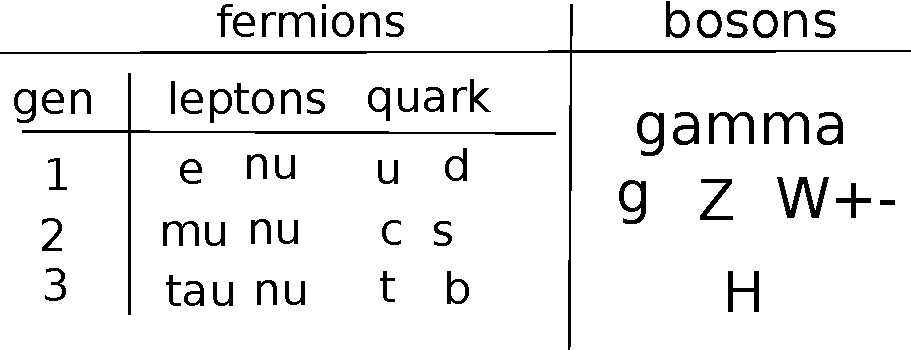
\includegraphics[width=.75\textwidth]{figurer/standard_model.pdf}
    \caption{The particles of the standard model}
    \label{fig: standard model}
\end{figure}


The part of the Standard Model which describes the interaction of quarks via the strong force, mediated by the gluons, is called \emph{quantum chromodynamics} (QCD).
Quarks are the building blocks of the nuclear particles, protons and neutrons, and the nuclear force that binds together atoms is a result of QCD.
A complete understanding of this theory is of great interest.
However, the fact that the force mediated by gluons is so strong greatly limits our understanding.
This is because our main technique for handling quantum field theories, perturbation theory, fails.
In perturbation theory, we rely on interactions being weak.
This is quantified by an expansion parameter, $\alpha$, to which the strength of each interaction is proportional.
If $\alpha<1$, then each such interaction in a process will suppress it by a factor $\alpha$.
The scattering of two particles is then calculated as a sum of all possible processes---combinations of interactions between the fields---that could lead to a scattering.
Processes with more interactions will contribute less to the total sum, as each interaction suppresses the diagram by $\alpha$.
Each process is illustrated by a Feynman diagram, in which particles come in from the left, interact via \emph{virtual particles}, then leave to the right.
The process of electron-electron scattering in quantum electrodynamics (QED) is given by
%
\begin{equation}
\begin{tikzpicture}[baseline=(c)]
    \begin{feynman}
        \vertex (a1) at (0, 0);
        \vertex (b1) at (1, 0);
        \vertex (c1) at (2, 0);
        %
        \vertex (a2) at (0, -1);
        \vertex (b2) at (1, -1);
        \vertex (c2) at (2, -1);
        %
        \vertex[left=0.1cm of a1] {$e^-$};
        \vertex[right=0.1cm of c1] {$e^-$};        
        \vertex[left=0.1cm of a2] {$\mu^-$};
        \vertex[right=0.1cm of c2] {$\mu^-$};
        %
        \node [blob] (c) at (1, -.5);
        %
        \diagram*{
            {[edges=fermion]
            (a1) -- (c) -- (c1),
            (a2) -- (c) -- (c2)},
        };
    \end{feynman}
\end{tikzpicture}
=
\underbrace{\, \,
 \begin{tikzpicture}[baseline=(c)]
    \begin{feynman}
        \vertex (a1) at (0, 0);
        \vertex (c1) at (2, 0);
        \vertex (a2) at (0, -1);
        \vertex (c2) at (2, -1);
        \vertex (x) at (1, -.2);
        \vertex (c) at (1, -.5);
        \vertex (y) at (1, -.8);
        \diagram*{
            {[edges=fermion]
            (a1) -- (x) -- (c1),
            (a2) -- (y) -- (c2)},
            {[edges=photon]
            (x) -- (y)}
        };
    \end{feynman}
\end{tikzpicture}
\, \,
}_{\propto \alpha}
+
\underbrace{ \, \,
\begin{tikzpicture}[baseline=(c)]
    \begin{feynman}
        \vertex (a1) at (0, 0);
        \vertex (d1) at (2.4, 0);
        \vertex (a2) at (0, -1);
        \vertex (d2) at (2.4, -1);
        \vertex (x) at (.8, -.2);
        \vertex (y) at (.8, -.8);
        \vertex (x2) at (1.6, -.2);
        \vertex (y2) at (1.6, -.8);
        \vertex (c) at (.8, -.5);
        \diagram*{
            {[edges=fermion]
            (a1) -- (x) -- (x2) -- (d1),
            (a2) -- (y) -- (y2) -- (d2)},
            {[edges=photon]
            (x) -- (y),
            (x2) -- (y2)}
        };
    \end{feynman}
\end{tikzpicture}
+
\begin{tikzpicture}[baseline=(c)]
    \begin{feynman}
        \vertex (a1) at (0, 0);
        \vertex (c1) at (2, 0);
        \vertex (a2) at (0, -1);
        \vertex (c2) at (2, -1);
        \vertex (x) at (1, 0);
        \vertex (l1) at (1, -.3);
        \vertex (c) at (1, -.5);
        \vertex (l2) at (1, -.7);
        \vertex (y) at (1, -1);
        \diagram*{
            {[edges=fermion]
            (a1) -- (x) -- (c1),
            (a2) -- (y) -- (c2),
            (l1) --[half left, looseness=1.8] (l2) --[half left, looseness=1.8] (l1),
            },
            {[edges=photon]
            (x) -- (l1),
            (l2) -- (y)
            }
        };
    \end{feynman}
\end{tikzpicture}
+
\begin{tikzpicture}[baseline=(c)]
    \begin{feynman}
        \vertex (a1) at (0, 0);
        \vertex (b1) at (.5, -.1);
        \vertex (c1) at (1, -.2);
        \vertex (d1) at (1.5, -.1);
        \vertex (e1) at (2, 0);
        \vertex (a2) at (0, -1);
        \vertex (c2) at (1, -.8);
        \vertex (e2) at (2, -1);
        \vertex (c) at (0, -.5);
        \diagram*{
            {[edges=fermion]
            (a1)--(c1)--(e1),
            (a2)--(c2)--(e2)},
            (b1) --[boson, quarter left] (d1),
            (c1) --[boson] (c2)
        };
    \end{feynman}
\end{tikzpicture}
\, \,
}_{\propto \alpha^2}
+ \dots
\end{equation}
%
In electrodynamics, the expansion parameter is the fine structure constant, $\alpha = e^2/(4 \pi)$ where $e$ is the elementary electrical charge.
In renormalized theories, such as QED, this parameter is dependent on the energy scale $Q$ the processes happen at.
This is called the running of a parameter.
At $Q = 0$, $ \alpha \approx 7 \times 10^{-3}$, and only a few orders in perturbation theory will therefore give highly precise and accurate results.
\footnote{
    The series expansion in terms of coupling constants is, strictly speaking, not a converging Taylor series, but rather an asymptotic series.
    We can see this by considering the consequences of exchanging $\alpha$ for $-\alpha$.
    Such a theory would be unstable like charges would attract.
    This implies any expansion in $\alpha$ has a zero radius of converge~\autocite{dysonDivergencePerturbationTheory1952}.
    We must therefore consider the sum of Feynman-diagrams as an asymptotic series, which yields a good approximation \emph{if terminated soon enough}~\autocite{floryHowLearnedStop2012}.
}

In QCD, we have no such luck.
The equivalent of the fine-structure constant in QCD, $\alpha_s$, increases as the energy scale decreases, in contrast to $\alpha$.
As a consequence, for $Q$ below around $1\,\text{GeV}$, perturbation theory breaks down.
This includes everything but the most extreme situations in the universe.
At such energy scales, quarks and gluons are bound together as \emph{hadrons}.
Hadrons are divided into two classes, \emph{baryons} and \emph{mesons}.
The nucleons---the neutron and the proton---are among the baryons.
Roughly, these are made up of three quarks, while the mesons are made of two.
The lightest meson, the pion, was predicted theoretically by Hideki Yukawa as the carrier of the nuclear force and later discovered by Cecil Powell \emph{et. al.}~\autocite{griffithsIntroductionElementaryParticles2008}

We are unable to directly and analytically describe QCD at low energies due to this breakdown of perturbation theory.
There are numerical schemes, namely lattice QCD, which allow for calculations of low energy QCD. \todo[]{sign problem + cost}
We will tackle the problem by using an \emph{effective field theory}.
When creating an effective field theory, we come to terms with the fact that we do not know all physics.
Instead, we settle for a description of the most important parts.
In modern physics, effective field theories have become a ubiquitous tool and are employed in both condensed matter physics and high-energy physics.
In fact, it is now believed that the Standard model itself is an effective field theory, a low energy description of a more complete theory~\autocite{pencoIntroductionEffectiveField2020,weinbergDevelopmentEffectiveField2021}.
The ``theorem'' Weinberg discusses in the opening quote of this chapter describes why effective field theories are such a powerful tool.
In short, it states that quantum field theories alone contain very little information, and thus can model almost everything.
If we write down the most general Lagrangian, then we have not made more than very basic assumptions~\autocite{weinbergPhenomenologicalLagrangians1979a}.
This will be our guiding philosophy when constructing chiral perturbation theory, the effective theory of mesons.



\section{The QCD phase diagram}

Pion stars are made up of condensed pions.
This is just one of the many phases of quantum chromodynamics.
A phase diagram illustrates what phases a medium is under different circumstances.
The phase diagram of QCD is rich and is an active area of research.
Our understanding of this phase diagram is far from complete due to the difficulties of working with the strong force.
\autoref{fig: phase diagram QCD} shows a rough sketch of our current understanding of the QCD phase diagram.
The axes are temperature $T$, baryon chemical potential $\mu_B$, and isospin chemical potential $\mu_I$.
The baryon and isospin chemical potentials quantify the abundance of quarks compared to  anti quarks and up quarks compared to down quarks, respectively.
Close to $T = \mu_B = \mu_I = 0$, QCD is in the vacuum phase, where hadrons form a gas whose density and composition depend on the temperature and chemical potentials.
Some of the first explorations of the phase transitions were done when it was CERN noticed that hadrons seem to approach a maximum temperature, the Hagedorn temperature of around $160\,\text{MeV}$ or $1.9\times 10^12 \, K$.
A more modern understanding of this temperature is as a point of phase transition, in which the quark ceases to be bound together as hadrons and instead forms a soup of free particles called quark-gluon plasma
This process is called deconfinement, and is a consequence of the weakening of the strong force for higher energies, called asymptotic freedom
~\autocite{hagedornHadronicMatterBoiling1968}\autocite{cabibboExponentialHadronicSpectrum1975}.
At zero isospin and barion chemical potential this transition, called a crossover, is smooth and characterized by a pseudo-critical temperature $T_{pc}$~\autocite{fukushimaPhaseDiagramDense2010}
Recent lattice QCD results indicate $T_{pc}$ is around $160\, \text{MeV}$.
Experimental observation of quark-gluon plasma was first reported by the Relativistic Heavy Ion Collider at Brookhaven National Laboratories in 2006~\autocite{adcoxFormationDensePartonic2005,backPHOBOSPerspectiveDiscoveries2005}.
\todo[]{Har vi nyere data?}

As the baryon chemical momentum increases, nucleons undergo a gass-liquid transition at low temperatures.
This happens approximately at the nuclear mass, $\mu_I \approx m_N \approx 0.9 \, \text{GeV}$.
As $\mu_B$ is turned up further, asymptotic freedom means that perturbative treatments again become available.
Under such conditions, QCD enters a phase analogous to electrical superconductors called \emph{color superconductor}.
Here, quarks at the surface of the Fermi sphere form Cooper pairs, as electrons do in the Bardeen-Cooper-Schrieffer (BCS) theory of electromagnetic superconductors.
Furthermore, there is a color Meissner effect, in which gluons gain mass due to the Higgs mechanism, as the photon does in electromagnetic superconductors.
The transition from the vacuum stater to the color superconducting state is not well understood.
Here, the density is still too low for perturbative treatment and numerical lattice calculations are haunted by the \emph{sign problem}.
QFT lattice methods discretize the fields on a finite lattice, representing space-time, then randomly sample configurations using the Metropolis-Hastings algorithm.
This, however, relies on each configuration having a real, positive weight which allows for the inclusion of a minority of important configurations.
For non-zero baryon chemical potential, this is not the case, and lattice methods therefore fail~\autocite{troyerComputationalComplexityFundamental2005}.

This problem does not arise in the case of zero baryon chemical potential, but a non-zero isospin chemical potential.
QCD lattice results, therefore, allow for an exploration of the behavior of QCD under non-zero $\mu_I$.
\chpt\, predicts a second order phase transition from the vacuum phase to a pion-condensed phase at $\mu_I = m_\pi$~\autocite{sonQCDFiniteIsospin2001}.
Early lattice calculations which agreed with these results~\autocite{kogutQuenchedLatticeQCD2002,kogutLatticeQCDFinite2002,kogutFiniteTemperatureTransition2004,sinclairSearchingElusiveCritical2006}, 
which have been confiremed by subsequent studies~\autocite{brandtNewClassCompact2018,brandtQCDFiniteIsospin2018,brandtQCDPhaseDiagram2018,brandtReliabilityTaylorExpansions2019,brandtQCDPhaseDiagram2017}.
The pion condensate is characterized by a non-zero condensate with an isospin charge.
This phase is a Bose-Einstein (BEC) phase, in which a zero-momentum state is higly occupied by identical bosons.
At asymptotically high $\mu_I$, it is conjectured that the BEC phase continuously transitions into a deconfined BSC state~\autocite{sonQCDFiniteIsospin2001a,sonQCDFiniteIsospin2001}.



\begin{figure}[!htb]
    \centering
    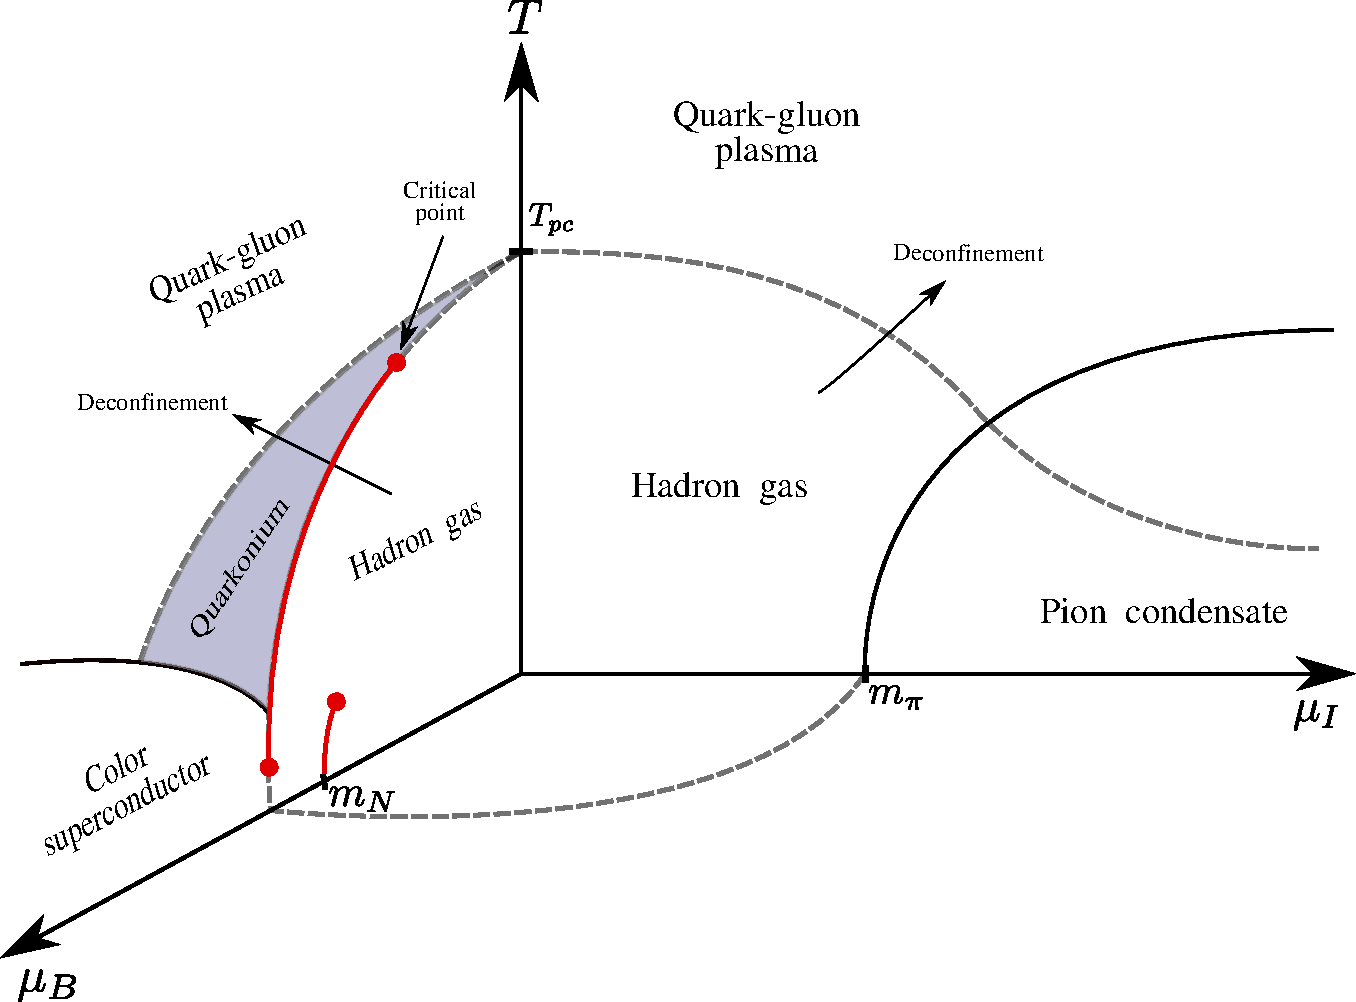
\includegraphics[width=.85\textwidth]{figurer/phase_diagram2.pdf}
    \caption{
        A scetch of the QCD phase diagram based on (KILDER)
        ~\autocite{fukushimaPhaseDiagramDense2010}\autocite{andronicHadronProductionUltrarelativistic2010}\autocite{baymHadronsQuarksNeutron2018}
        }
    \label{fig: phase diagram QCD}
\end{figure}






\section{Units}
\label{section: units}


In this thesis, we employ \emph{natural units}, defined by
%
\begin{equation}
    \hbar = c = k_B = 1,
\end{equation}
%
where $\hbar$ is Planck's reduced constant, $c$ is the speed of light, and $k_B$ is Boltzmann's constant.
Dimensionfull results are often given in $\text{MeV}$.
Uncertainties are indicated when the precision is less than four significant figures. 
However, the central value is always used in calculations.
All values in this section are from the Particle Data Group~\cite{particledatagroupReviewParticlePhysics2020}.
To obtain results in the SI-system, we use the following conversion factors, as given by
%
\begin{align}
    \label{speed of ligh}
    c       &= 2.998 \cdot 10^8     \, \text{m} \, \text{s}^{-1}, \\
    \label{hbar}
    \hbar   &= 1.055 \cdot 10^{-34} \, \text{J} \, \text{s}, \\
    \label{Boltzmanns constat}
    k_B     &= 1.380 \cdot 10^{-23} \, \text{J} \, \text K^{-1}, \\
    \label{Newtons gravitational constant}
    G       &= 6.674 \cdot 10^{-11} \, \text m^3 \, \text{kg}^{-1} \, \text s^{-2},
\end{align}
%
where $G$ is Newton's gravitational constant.
The conversion factor between $\text{MeV}$ and SI-units is
%
\begin{equation}
    \label{electronvolt}
    1 \, \text{MeV} = 1.60218\, \cdot 10^{-19} \, \text{J}. 
\end{equation}
%
The fine structure constant and the elementary charge is
%
\begin{align}
    \label{Fine structure constant}
    \alpha &= 7.297 \cdot 10^{-3}, \\
    \label{Elementary charge}
    e &:= \sqrt{4 \pi \alpha} =  3.028\cdot 10^{-1}.
\end{align}
%
In astronomical calculation, the solar mass is used, which is
%
\begin{equation}
    \label{solar mass}
    M_\odot = 1.988 \cdot 10^{30} \, \text{kg}.
\end{equation}
%
The physical parameters we use are
%
\begingroup
\allowdisplaybreaks % Make page break possbible
\begin{align}
    \label{pion decay constant}
    f_\pi & =  92.1 \, \text{MeV}, \\
    \label{pion mass}
    m_\pio & = 134.98 \, \text{MeV}, \\
    \label{charged pion mass}
    m_{\pipm} &= 139.57 \, \text{MeV}, \\
    m_{\Kpm} & = 493.68\,\text{MeV}, \\
    m_{\Ko} & = 497.61\,\text{MeV}, \\
    m_e &= 0.5110 \, \text{MeV}, \\
    m_\mu &= 105.7 \, \text{MeV}, \\
    \label{mass of neutron}
    m_N &= 939.57 \, \text{MeV}.
\end{align}
\endgroup

To make this thesis as self-contained as possible, we have included some parts from the earlier specialization project, with minor modifications.
These sections are marked with an asterisk in the table of content.
